\providecommand{\main}{../..}
\documentclass[\main/thesis.tex]{subfiles}

\begin{document}

\section{Equilibrium}
To test that the model can maintain tissue such that the cell numbers stay at equilibrium and tumours do not sporadically appear without carcinogens, we run a simulation that does not include any carcinogens. This will show that in our base model, random mutations alone cannot cause cancer to form due to the low mutational rate of genes in the body, and the fact that the body is well adept at fixing mutations as they occur. We run the simulation on a 128${\times}$128 grid for 8766 time-steps, and as stated above, with no carcinogens. 

In Figure \ref{fig:EquilibriumTimeSteps} we present three time-steps from a simulation where no carcinogens were included, with NTC as the brown cells, NSC as the blue cells, and empty cells are white. The Figures \ref{fig:EquilibriumTimeSteps} show (a) the initial seed, (b) the domain (tissue) at the halfway point of the simulation, and (c) the final time-step. 
We observe that the tissue stayed in equilibrium. The changes through time are due to cell movement and the natural birth and death processes. The figures show that, as desired, no mutated cells (green, yellow) arise and thus no cancer stem cells (purple) or tumour cells (red) are formed. 
\begin{figure}[H]
    \centering
    \begin{subfigure}[t]{.3\textwidth}
        \centering
        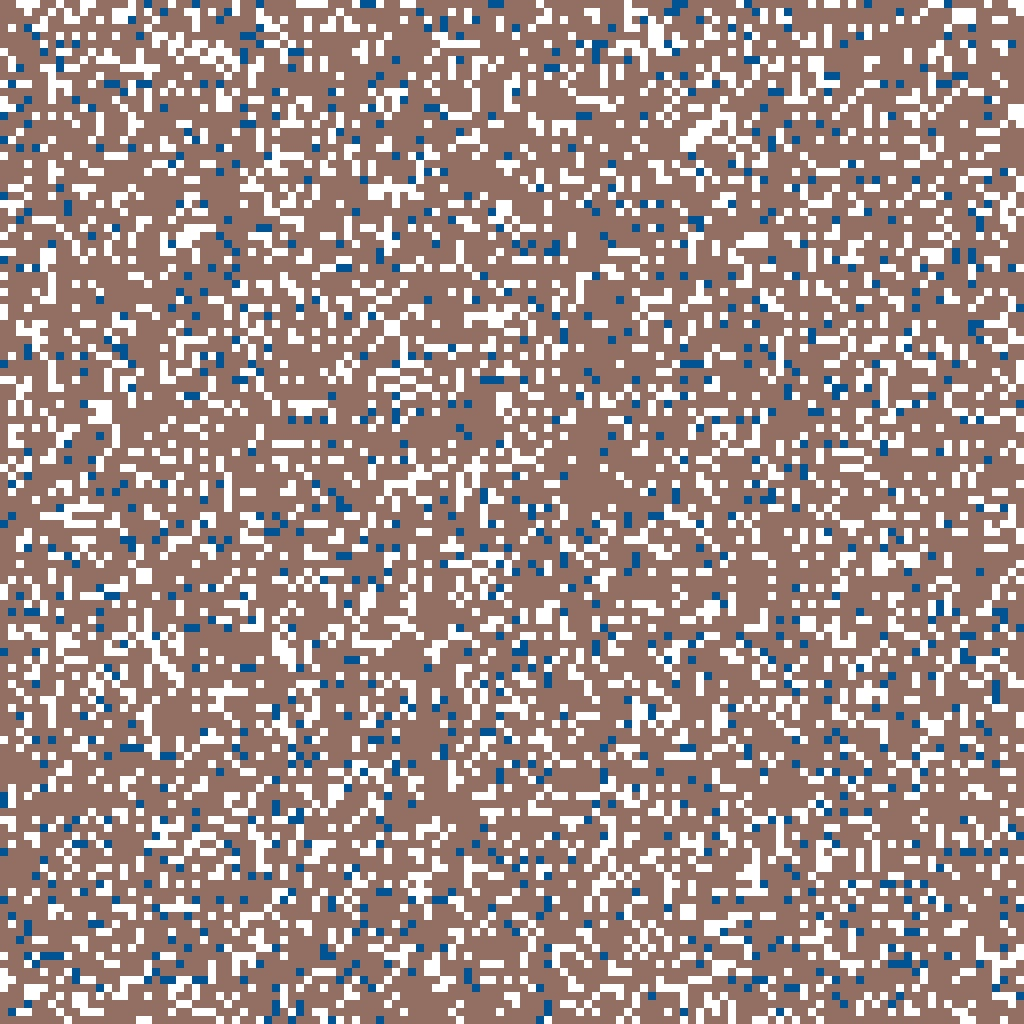
\includegraphics[width=\textwidth]{images/1_Equilibrium/Fig2/1_initial_seed.jpeg}
        \caption{Initial Seed}
        \label{fig:EquilibriumInitalSeed}
    \end{subfigure}
    \hfill
    \begin{subfigure}[t]{.3\textwidth}
        \centering
        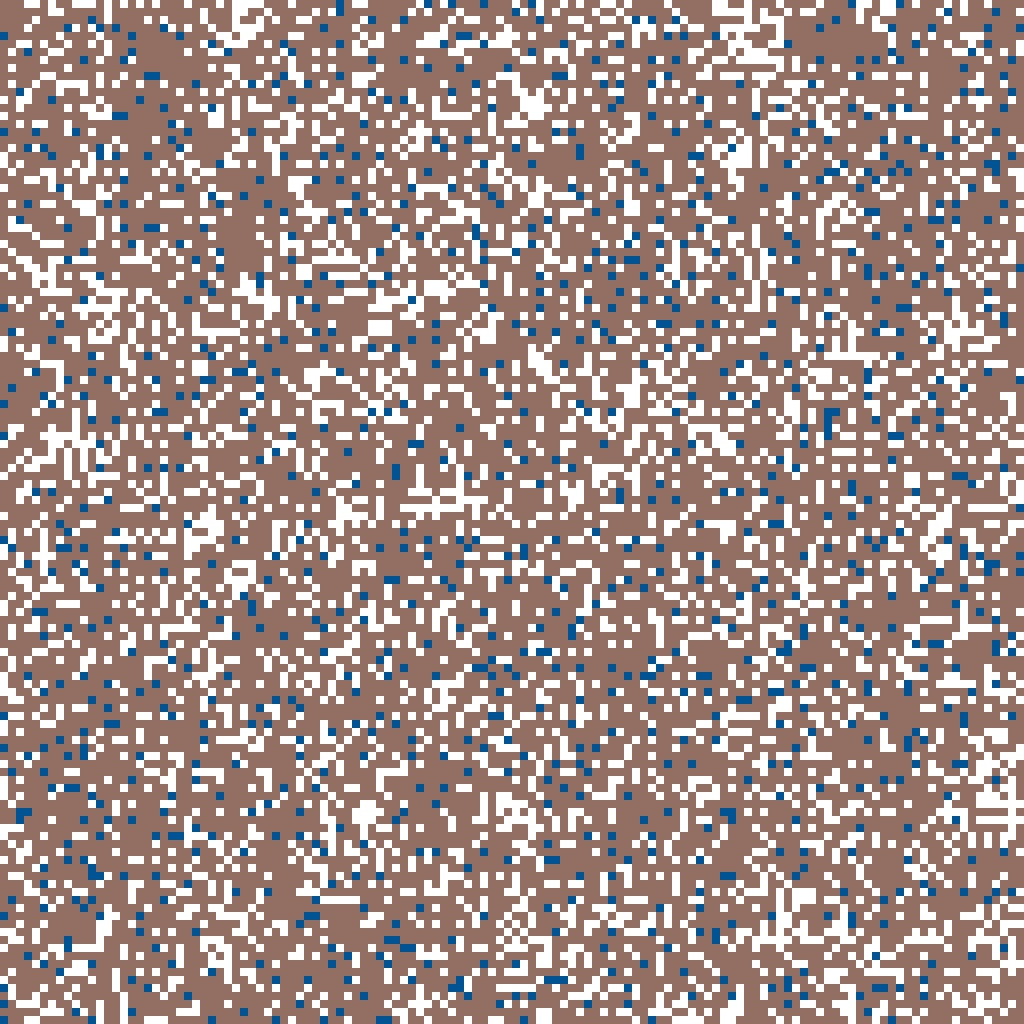
\includegraphics[width=\textwidth]{images/1_Equilibrium/Fig2/2_halfway_time_step.jpeg}
        \caption{Time-step 4383 (5 years)}
        \label{fig:EquilibriumHalwayPoint}
    \end{subfigure}
    \hfill
    \begin{subfigure}[t]{.3\textwidth}
        \centering
        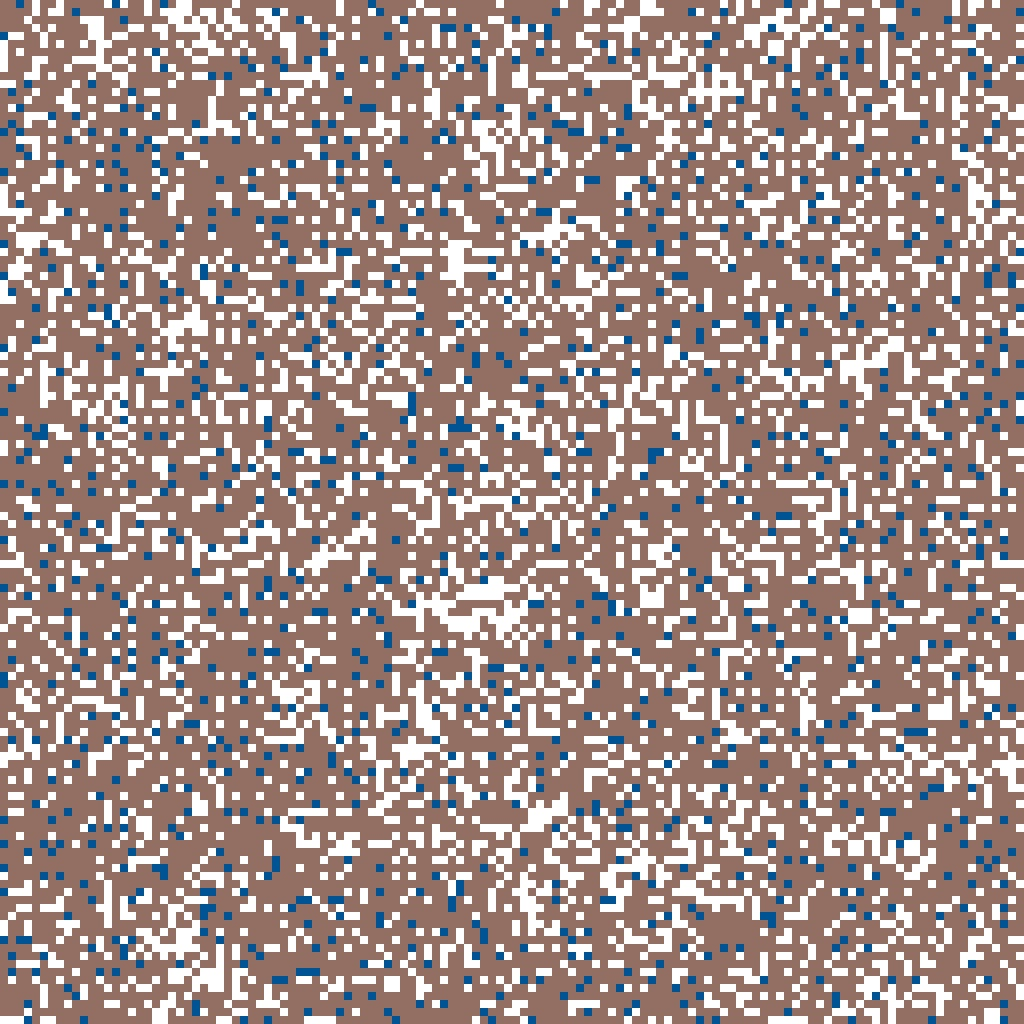
\includegraphics[width=\textwidth]{images/1_Equilibrium/Fig2/3_last_time_step.jpeg}
        \caption{Time-step 8766 (10 years)}
        \label{fig:EquilibriumFinalTimeStep}
    \end{subfigure}
    \caption{This figure includes three time-steps from a simulation with parameters set at: grid size 128x128 and no active carcinogens. Using the colour map for the cell classes as provided in Table \ref{table:CAStates}. These show (a) the initial seed of the simulation, in (b) the domain (tissue) at the halfway point of the simulation, and in (c) the final time-step.}
    \label{fig:EquilibriumTimeSteps}
\end{figure}

In Figure \ref{fig:EquilibriumNumState} we present the time evolution of the fraction of cells in the different cell classes. We see that the fraction of normal tissue stays constant (with small fluctuations) and mutated cell classes never form. Figure \ref{fig:EquilibriumNumState} shows us that, as desired, the number of NSC and NTC stay approximately constant over time. 
\begin{figure}[H]
    \centering
    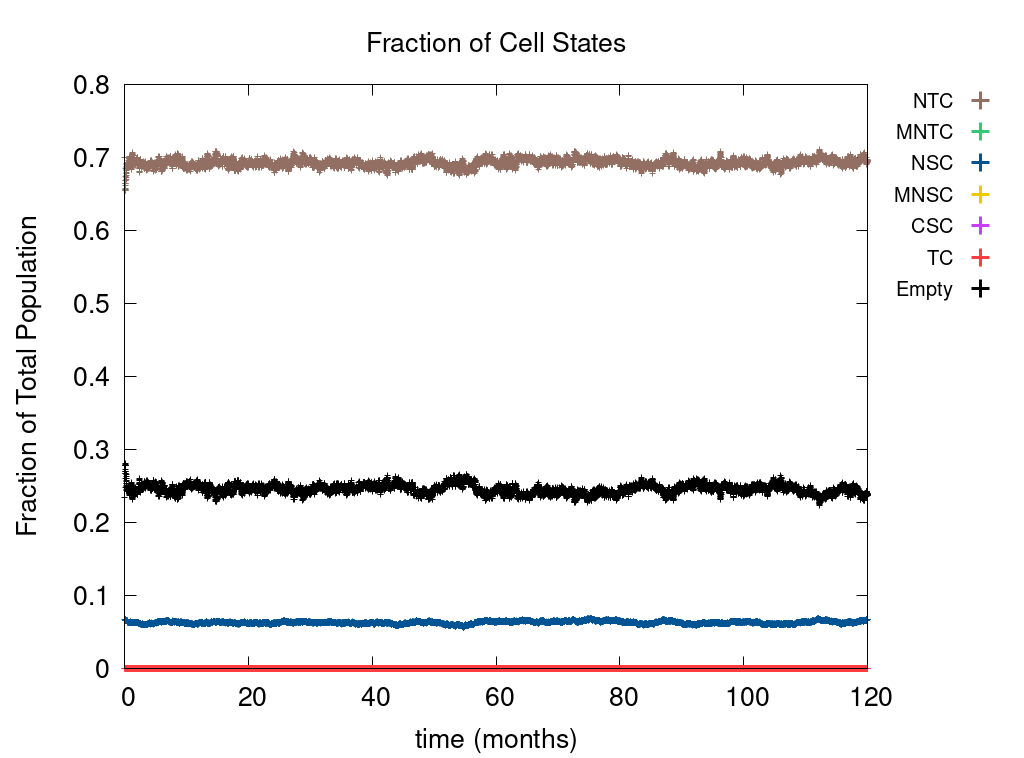
\includegraphics[width=\textwidth]{images/1_Equilibrium/Fig1/numState_all.png}
    \caption{This figure shows the time course of the fraction of cells in the different cell classes NTC, MNTC, NSC, MNSC, CSC, TC, and empty. The parameters of the simulation were as follows: grid size was 128x128 and no carcinogens were active.}
    \label{fig:EquilibriumNumState}
\end{figure}

In Figure \ref{fig:EquilibriumGeneExprAll} we present the time evolution of the average gene expression for each of the ten genes. We see that all of the genes maintain a normal gene expression of zero. This does not necessarily mean that the cells had a zero gene expression, but those that did were negligible due to the averaging process. We can see that none of the genes are mutated. Our model is able to maintain regular healthy tissue. 
\begin{figure}[H]
    \centering
    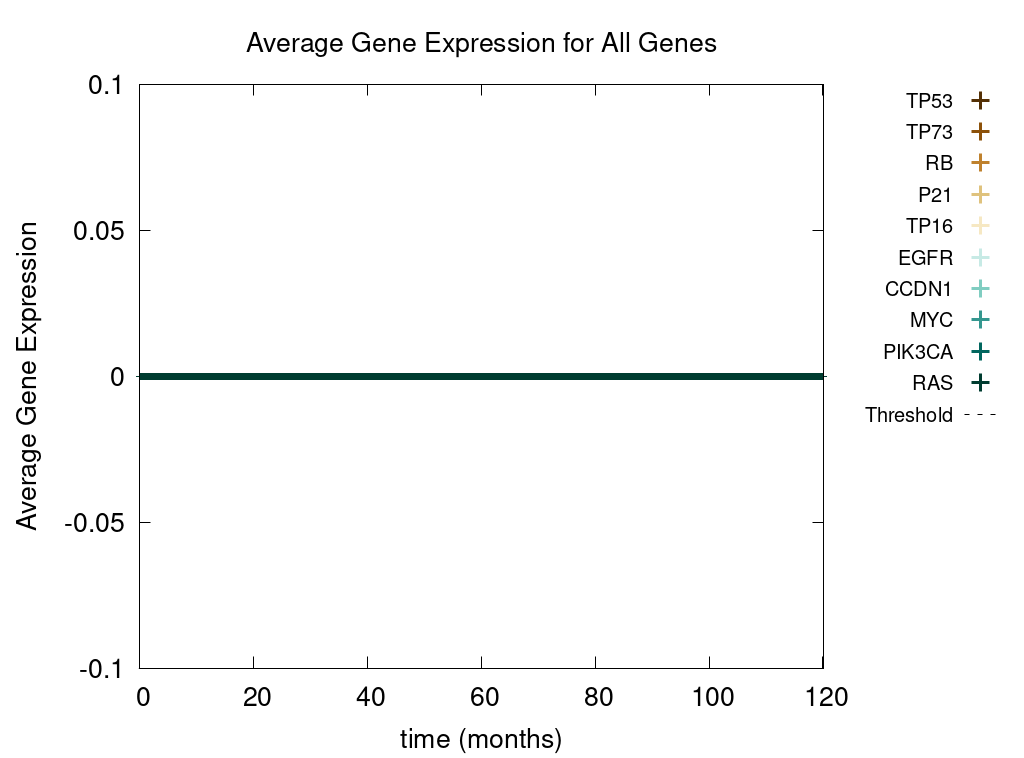
\includegraphics[width=\textwidth]{images/1_Equilibrium/Fig3/geneExprAll_all.png}
    \caption{This figure shows the time course of the average gene expression for the ten genes we consider. The parameters of the simulation were as follows: grid size was 128x128 and no carcinogens were active.}
    \label{fig:EquilibriumGeneExprAll}
\end{figure}

\end{document}